\begin{flushright} {\tiny {\color{gray} \tt pair\_raviart\_thomas.tex}} \end{flushright}
%~~~~~~~~~~~~~~~~~~~~~~~~~~~~~~~~~~~~~~~~~~~~~~~~~~~~~~~~~~~~~~~~~~~~~~~~~~~~~~~~~~~~~~~~~~~~~~~~~~

\subsection{What the literature says}

This element is substantially more complicated than most of the others
in FieldStone so I have proceeded systematically by 
scanning the literature (i.e. textbooks mostly) for 
useful definitions and statements. What follows is mostly a collection
of relevant/interesting statements.  



\begin{itemize}

%%%%%%%%%%%%%%%%%%%%%%%%%%%%%%%%%%%%%%%%%%%%%%%%%%%%%%%%%%%%%%%%%%%%%%%%%%%%%%%
\item 
There is an entire chapter (14) of \textcite{ergu21_72} dedicated to 
Raviart-Thomas elements and $H(\text{div})$.
%%%%%%%%%%%%%%%%%%%%%%%%%%%%%%%%%%%%%%%%%%%%%%%%%%%%%%%%%%%%%%%%%%%%%%%%%%%%%%%
\item 
Likewise Chapter 3 of \textcite{gatica} is dedicated to Raviart-Thomas spaces.

%%%%%%%%%%%%%%%%%%%%%%%%%%%%%%%%%%%%%%%%%%%%%%%%%%%%%%%%%%%%%%%%%%%%%%%%%%%%%%%
\item 
Conerning the Stokes equations, 
I have found a reference\footnote{\url{https://lyc102.github.io/ifem/fem/StokesRT0femrate/}}
that uses the stable element RT0-P0 (the lowest order Raviart-Thomas element for velocity 
and piecewise constant for pressure) of Stokes equations in 2-D.
In \textcite{lelk15} (2015) we read:
\begin{displayquote}
{\color{darkgray}
As shown in \cite{kans08} for the isoviscous case, the $RT_0-P_0$ element in the 
corresponding numerical scheme resembles the finite difference (FD) staggered grid 
stencil. Raviart-Thomas elements of order $k$ can, therefore, be considered a higher-order
generalization of the FD method working on irregular meshes.
}
\end{displayquote}
Note that the authors compare $Q_1\times P_0$, $Q_2 \times P_{-1}$, $RT_0-P_0$ and 
$BDM_1-P_0$ for the Stokes equation but the two last ones rely on DG. 

Interestingly enough, the RT elements are described in \cite{aubb17} but 
only used for thermal problems, not Stokes, while other elements are proposed 
for Stokes. Could it be bc for RT0-P0 on quads we have $\dot{\varepsilon}^h_{xy}=0$
due to the formulation of the basis functions ? Is this why \cite{lelk15}
use it in DG formulation and not CG?

 
%%%%%%%%%%%%%%%%%%%%%%%%%%%%%%%%%%%%%%%%%%%%%%%%%%%%%%%%%%%%%%%%%%%%%%%%%%%%%%%
\item 
In \textcite{hald03} (2003) we find: 
\begin{displayquote}
{\color{darkgray}
$P_1^\perp \times P_0$ symbol denotes an element with 
normal velocity nodes in the middle of each edge of the
triangulation [...]. This element, also called low order Raviart–Thomas element 
(Raviart and Thomas, 1977 \cite{rath77}), is based on flux conservation on elements edges and 
the resulting scheme is very close to a finite volume scheme.
}
\end{displayquote}

%%%%%%%%%%%%%%%%%%%%%%%%%%%%%%%%%%%%%%%%%%%%%%%%%%%%%%%%%%%%%%%%%%%%%%%%%%%%%%%
\item 
It is mentioned in \textcite{john16}, appendix B.3, example B.45: 
\begin{displayquote}
{\color{darkgray}
the normal component of v 
on each face is a constant. The normal component of functions from RT0 is
continuous across faces of the mesh cells.
}
\end{displayquote}


%%%%%%%%%%%%%%%%%%%%%%%%%%%%%%%%%%%%%%%%%%%%%%%%%%%%%%%%%%%%%%%%%%%%%%%%%%%%%%%
\item
In \textcite{chen93a} (1993) we read:
\begin{displayquote}
{\color{darkgray}
Arnold and Brezzi [2] showed, for
example, that the Raviart-Thomas mixed method of lowest order is
equivalent to the usual $P_1$-nonconforming method modified by augmenting
the classical $P_1$-nonconforming space with $P_3$-bubbles and then proved that
the equivalence is useful not only for implementing the mixed method but
also for deriving error estimates.
}
\end{displayquote}


%%%%%%%%%%%%%%%%%%%%%%%%%%%%%%%%%%%%%%%%%%%%%%%%%%%%%%%%%%%%%%%%%%%%%%%%%%%%%%%
\item
There is an entry on Wikipedia\footnote{\url{
https://en.wikipedia.org/wiki/Raviart-Thomas_basis_functions
}} but it is short and not so useful, except for
\begin{displayquote}
{\color{darkgray}
In applied mathematics, Raviart–Thomas basis functions are vector basis functions used 
in finite element and boundary element methods. They are regularly used as basis 
functions when working in electromagnetics. 
}
\end{displayquote}

%%%%%%%%%%%%%%%%%%%%%%%%%%%%%%%%%%%%%%%%%%%%%%%%%%%%%%%%%%%%%%%%%%%%%%%%%%%%%%%
\item
There is also a useful entry on Stackexchange\footnote{\url{
https://scicomp.stackexchange.com/questions/20245/raviart-thomas-elements-on-reference-square}}:
\begin{displayquote}
{\color{darkgray}
There are quadrilateral Raviart-Thomas elements. 
In two dimensions, the polynomial space for $RT_k$ is given by 
$P_{k+1,k} \times P_{k,k+1}$, where
\[
P_{k,l}=\left\{ \sum_{i=0}^{k} \sum_{j=0}^{l} a_{ij} x^i y^j: a_{ij}\in \R  \right\}
\]

A typical polynomial for $k=0$ would thus be 
\[
\left(
\begin{array}{c}
a_1+b_1 x \\
a_2+b_2 y
\end{array}
\right)
\]
and for $k=1$:
\[
\left(
\begin{array}{c}
a_1+b_1 x +c_1x^2 +d_1 y + e_1 xy  + f_2 x^2 y\\
a_2+b_2 y +c_2y^2 +d_2 x + e_2 xy  + f_2 x y^2
\end{array}
\right)
\]
Hence, $dim(RT_1)=12$, and in general, $dim(RT_k)=2(k+1)(k+2)$. 
This means you need two additional degrees of freedom, which should be located on the 
interior of the element. (In general, for $RT_k$ you take $k+1$ normal derivatives on each facet, 
and the remaining degrees of freedom from the interior.)

For Raviart-Thomas elements, you usually take moments rather than 
point evaluations, i.e., the remaining conditions come from the conditions 
\[
\int_{-1}^{+1} \int_{-1}^{+1} \phi_i(x,y)q_j(x,y)dx dy = \delta_{ij}
\]
where the ${q_j}$ are a basis of $P_{k-1,k}\times P_{k,k-1}$ (e.g. $1,x,y$ for $k=1$).
To make it easier to get a full nodal basis, the facet degrees of freedom are 
usually not taken as point evaluation, but also as moment conditions: 
\[
\int_{e_m} \phi_i(s)^T \nu_{e_m} q_{m,j}(s) ds
\]
where $e_m$ is one of the four edges, $\nu_{e_m}$ is the corresponding outer normal, 
and for each $m$, the $q_{m,j}$ form a basis of $P_k(e_m)$ (e.g. {1,x} or {1,y}
for $k=1$ depending on the edge orientation).
Together, these degrees of freedom are unisolvent (i.e., the corresponding system 
of basis functions is always invertible).
}
\end{displayquote}



%%%%%%%%%%%%%%%%%%%%%%%%%%%%%%%%%%%%%%%%%%%%%%%%%%%%%%%%%%%%%%%%%%%%%%%%%%%%%%%
\item
In \textcite{kanschat17}  we find:
\begin{displayquote}
{\color{darkgray}

The Raviart-Thomas element of degree $k\ge 0$ on
simplices consists of the polynomial space
\[
RT_k = {\mathbb P}_k^d + x {\mathbb P}_k.
\]

For the simplicial Raviart-Thomas element in $\R^d$
there holds
\[
dim(RT_k) = (d+1) dim({\mathbb P}_k) - dim({\mathbb P}_{k-1})
\]
In particular:
\begin{eqnarray}
dim(RT_k)|_{2D} &=& (k+1)(k+3) \nn\\
dim(RT_k)|_{3D} &=& \frac12(k+1)(k+2)(k+4)\nn
\end{eqnarray}


\begin{center}
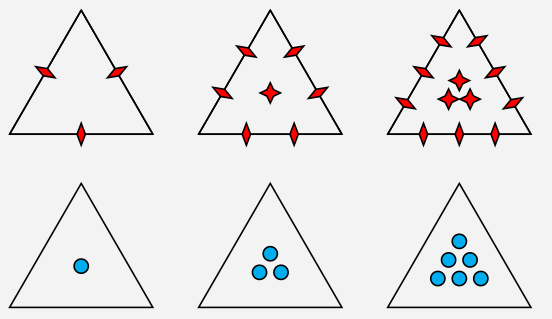
\includegraphics[width=6.7cm]{images/pair_raviart-thomas/RT_kanschat_T}
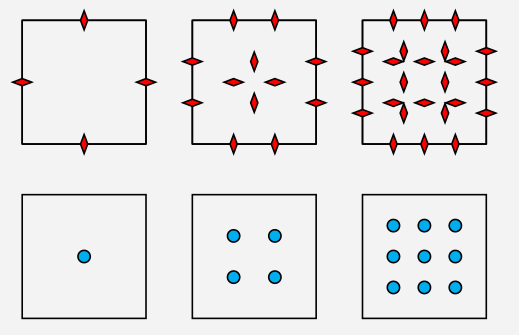
\includegraphics[width=6cm]{images/pair_raviart-thomas/RT_kanschat_Q}\\
{\captionfont Examples 4.2.10 and 4.2.37 of \textcite{kanschat17}.
The first members of the Raviart-Thomas family on triangles and quadrilaterals.
}
\end{center}

The construction principle of the Raviart-Thomas element on simplices as well
as on rectangles and cubes can be seen as adding vector polynomials to the
velocity space until its divergence is equal to ${\mathbb P}_k$ or ${\mathbb Q}_k$ .

The Raviart-Thomas element of degree $k\ge 0$
on the reference cell $\hat{T}=[-1,1]^d$ consists of the polynomial space
\[
RT_k(\hat{T}) = {\mathbb Q}_k^d(\hat{T}) + x {\mathbb Q}_k(\hat{T})
\]
and we have
\[
dim(RT_k) = d(k+1)^{d-1}(k+2)
\]

}
\end{displayquote}

%%%%%%%%%%%%%%%%%%%%%%%%%%%%%%%%%%%%%%%%%%%%%%%%%%%%%%%%%%%%%%%%%%%%%%%%%%%%%%%
\item
This element is implemented in deal.II and we 
read\footnote{\url{https://www.dealii.org/current/doxygen/deal.II/classFE__RaviartThomas.html}}:
\begin{displayquote}
{\color{darkgray}
The Raviart-Thomas space is designed to solve problems in which the solution only 
lives in the space $H^{\text{div}}=\{ {\bm u} \in L_2 :\text{div}({\bm u}) \in L_2\}$, 
rather than in the more commonly used space $H^1=\{ {\bm u} \in L_2 : \nabla {\bm u} \in L_2 \}$. 
In other words, the solution must be a vector field whose divergence is square integrable, 
but for which the gradient may not be square integrable. The typical application for this space 
(and these elements) is to the mixed formulation of the Laplace equation and related situations, 
see for example step-20. The defining characteristic of functions in  $H^{\text{div}}$ is that they are 
in general discontinuous - but that if you draw a line in 2d (or a surface in 3d), 
then the normal component of the vector field must be continuous across the line (or surface) 
even though the tangential component may not be. As a consequence, the Raviart-Thomas element 
is constructed in such a way that (i) it is vector-valued, (ii) the shape functions are 
discontinuous, but (iii) the normal component of the vector field represented by each shape 
function is continuous across the faces of cells.

Other properties of the Raviart-Thomas element are that 
(i) it is not a primitive element; (ii) the shape functions are defined so that 
certain integrals over the faces are 
either zero or one, rather than the common case of certain point values being 
either zero or one. 

We follow the commonly used - though confusing - definition of the ``degree'' of RT elements. 
Specifically, the ``degree'' of the element denotes the polynomial degree of the 
largest complete polynomial subspace contained in the finite element space, 
even if the space may contain shape functions of higher polynomial degree. 
The lowest order element is consequently FE\_RaviartThomas(0), i.e., 
the Raviart-Thomas element ``of degree zero'', even though the functions of this space 
are in general polynomials of degree one in each variable. This choice of ``degree'' 
implies that the approximation order of the function itself is degree+1, as with usual polynomial spaces. 
}
\end{displayquote}

%%%%%%%%%%%%%%%%%%%%%%%%%%%%%%%%%%%%%%%%%%%%%%%%%%%%%%%%%%%%%%%%%%%%%%%%%%%%%%%
\item 
Elsewhere in the deal.II library\footnote{\url{https://www.dealii.org/current/doxygen/deal.II/classPolynomialsRaviartThomas.html}} we read\footnote{Note that at the time deal.II only supported quads.}
\begin{displayquote}
{\color{darkgray}
The Raviart-Thomas polynomials are constructed such that the divergence is 
in the tensor product polynomial space $Q_k$. Therefore, the polynomial order of each component 
must be one order higher in the corresponding direction, yielding the polynomial spaces 
$(Q_{k+1,k}, Q_{k,k+1})$ and $(Q_{k+1,k,k}, Q_{k,k+1,k}, Q_{k,k,k+1})$ in 2d and 3d, respectively. 
}
\end{displayquote}

The Raviart-Thomas element is used in Step-20 (\url{https://www.dealii.org/current/doxygen/deal.II/step_20.html}) and Step-21 (\url{https://www.dealii.org/current/doxygen/deal.II/step_21.html}).


%%%%%%%%%%%%%%%%%%%%%%%%%%%%%%%%%%%%%%%%%%%%%%%%%%%%%%%%%%%%%%%%%%%%%%%%%%%%%%%
\item
In John's book \cite{john16} we find:
\begin{displayquote}
{\color{darkgray}
Raviart–Thomas finite elements are a class of vector-valued finite elements that approximate the space
$H(\text{div},\Omega)=\{ {\bm v} \in L^2(\Omega): \nabla \cdot {\bm v} \in L^2(\Omega)  \}$.
Details of their definition and important properties can be
found, e.g., in page 84 of \textcite{bobf13} (2013).

Consider a simplicial triangulation with mesh cells $\{K\}$ and let ${\bm P}_k(K)=(P_k(K))^d$, $k\ge 0$.
Then, the following local polynomial space is defined directly on $K$:
\[
RT_k(K)=\{ {\bm v} \in ({\bm P}_k(K) + {\bm x} P_k(K)) : 
{\bm v}\cdot{\bm n}_{\partial K} \in R_k(\partial K)\},
\qquad k\ge 0,
\]
where
\[
R_k(\partial K)=\{ \phi \in L^2(\partial K): \phi|_E\in P_k(E) \text{ for all faces } E\subset \partial K \}
\]
It is noted in \textcite{bobf13} (remark 2.3.1) that this definition of $RT_k(K)$
is different than the original definition in \textcite{rath77} (1977).

In particular, the Raviart-Thomas element of lowest order is given by
\[
RT_0(K)=\{ {\bm v} \in ({\bm P}_0(K)+{\bm x} P_0(K)) : {\bm v} \cdot {\bm n}_{\partial K} \in R_0(\partial K)  \}
\]
i.e., it is linear on $K$. Its local functionals are ${\bm v} \cdot {\bm n}_{E_i}$, $i=1,..d+1$. 
A function from $RT_0(K)$ can be written in the form
\[
{\bm v}({\bm x}) = {\bm a} + b {\bm x}, \quad {\bm a}\in \R^d, b\in \R, {\bm x}\in K. \qquad B.21
\]
A face $E\subset \partial K$ is a hyperplane that can be represented in the form
\[
{\bm x}\cdot {\bm n}_E = c, \qquad c\in \R, \forall {\bm x} \in E.
\]
Inserting this representation in (B.21) yields
\[
{\bm v}({\bm x})\cdot {\bm n}_E = {\bm a}\cdot {\bm n}_E + b {\bm x} \cdot {\bm n}_E = {\bm a}\cdot {\bm n}_E + bc =const
\qquad \forall {\bm x}\in E.
\]
Thus, the normal component of ${\bm v}$ on each face is a constant.

}
\end{displayquote}



%%%%%%%%%%%%%%%%%%%%%%%%%%%%%%%%%%%%%%%%%%%%%%%%%%%%%%%%%%%%%%%%%%%%%%%%%%%%%%%
\item 
On the defelement site\footnote{\url{https://defelement.com/elements/raviart-thomas.html}} we find 
that it is defined on triangles, tetrahedra, quadilaterals and hexahedra.
with the number of dofs defined as follows:
\begin{itemize}
\item triangle: $k(k+2)$
\item tetrahedron: $k(k+1)(k+3)/2$
\item quadrilateral: $2k(k+1)$
\item hexahedron: $3k^2(k+1)$
\end{itemize}

%%%%%%%%%%%%%%%%%%%%%%%%%%%%%%%%%%%%%%%%%%%%%%%%%%%%%%%%%%%%%%%%%%%%%%%%%%%%%%%
\item
In \textcite{brfo} (1991) we read:

\begin{displayquote}
{\color{darkgray}
On triangles we know that $RT_0$ is a space of dimension 3 containing polynomials of the form
\begin{eqnarray}
q_1(x,y)&=&a+cx \nn\\
q_2(x,y)&=&b+cy \nn
\end{eqnarray}

\begin{center}
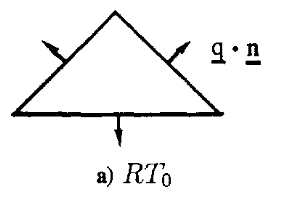
\includegraphics[width=3cm]{images/pair_raviart-thomas/brfo1}
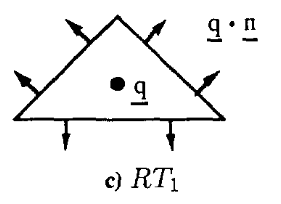
\includegraphics[width=3cm]{images/pair_raviart-thomas/brfo2}
\end{center}
The simplest cases of three-dimensional elements are depicted here:
\begin{center}
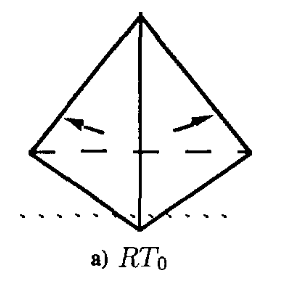
\includegraphics[width=3cm]{images/pair_raviart-thomas/brfo3}
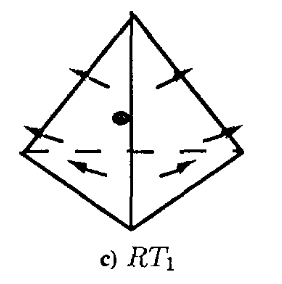
\includegraphics[width=3cm]{images/pair_raviart-thomas/brfo4}
\end{center}

We now consider the extension of the previous construction to rectangular 
elements
In the present case, the use of a reference element is essential and we shall build
our space on $\hat{K}=]-1,1[^n$. Contrarily to the simplicial case, it will be
simpler here to first introduce the approximations of Raviart and Thomas.
Let us thus define, as in the previous section,
\[
RT_{[k]} = (Q_k)^n + \underline{x} Q_k
\]
It can be checked that one has
\begin{eqnarray}
RT_{[k]}|_{n=2} &=& P_{k+1,k} \times P_{k,k+1} \nn\\
RT_{[k]}|_{n=3} &=& P_{k+1,k,k} \times P_{k,k+1,k} \times P_{k,k,k+1} \nn
\end{eqnarray}
and 
\[
dim(RT_{[k]}|_{n=2}) = 2(k+1)(k+2)
\]
\[
dim(RT_{[k]}|_{n=3}) = 3(k+1)^2(k+2)
\]

}
\end{displayquote}



%%%%%%%%%%%%%%%%%%%%%%%%%%%%%%%%%%%%%%%%%%%%%%%%%%%%%%%%%%%%%%%%%%%%%%%%%%%%%%%
\item
In \textcite{LarsonBengzon} we read: 
\begin{displayquote}
{\color{darkgray}
Not all finite elements are scalar and there are also vector valued elements. As
the name suggests, vector valued elements are used to approximate vector valued
functions. One such element is the Raviart-Thomas element, which is designed to
mimic the Hilbert space
\[
H(\text{div}; \Omega) = \{ v\in [L^2(\Omega)]^2 : \nabla \cdot v \in L^2(\Omega) \}
\]
That is, the space of all vectors with bounded divergence. A simple application
of Green’s formula shows that all such functions must have continuous normal
components, which is the basic design feature of the Raviart-Thomas element.



Actually there is a whole family of Raviart Thomas elements, but we shall only
study the simplest of them called the RT0 element. On a triangle $K$ the polynomial
space for $RT_0$ is given by $P=[P_0(K)]^2 + [x_1,x_2]^T P_0(K)$
, that is, all vectors of the form 
\[
v = \left[ \begin{array}{c} a_1 \\ a_2 \end{array} \right]
+ b\left[ \begin{array}{c} x_1 \\ x_2 \end{array} \right]
\]
for some coefficients $a_1$ , $a_2$ , and $b$.

If the normal is chosen consistently on each edge in the mesh, then by
construction is the $RT_0$ shape functions are continuous in the normal direction
across the edge of any two adjacent elements. This ensures that the $RT_0$ functions
belong to $H(\text{div},\Omega)$.

The isoparametric map can not be used for $RT_0$ elements, since the divergence
is not preserved by this mapping.

The Raviart-Thomas elements typically find application in acoustics and
elasticity.

\begin{center}
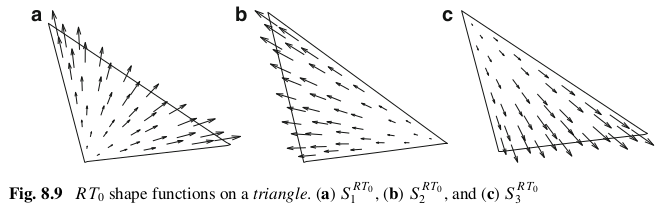
\includegraphics[width=11cm]{images/pair_raviart-thomas/larsonbengzon}
\end{center}

}
\end{displayquote}

%%%%%%%%%%%%%%%%%%%%%%%%%%%%%%%%%%%%%%%%%%%%%%%%%%%%%%%%%%%%%%%%%%%%%%%%%%%%%%%
\item
In \textcite{lomw12} we find:
\begin{displayquote}
{\color{darkgray}
The Sobolev space $H(\text{div})$ consists of vector fields for which the 
components and the weak divergence are square-integrable. This is a 
weaker requirement than for a $d$-vector field to be in $[H^1]^d$ (for $d\ge 2$).
This space naturally occurs in connection with mixed formulations 
of second-order elliptic problems,
porous media flow, and elasticity equations. For a finite element 
family to be $H(\text{div})$-conforming, each component need not be continuous, 
but the normal component must be continuous. In order
to ensure such continuity, the degrees of freedom of $H(\text{div})$-conforming 
elements usually include normal components on element facets.
The two main families of $H(\text{div})$-conforming elements are the Raviart–Thomas 
and Brezzi-Douglas-Marini elements.

The Raviart–Thomas element was introduced by Raviart and Thomas (1977) \cite{rath77}. 
It was the first element to discretize the mixed form of second-order 
elliptic equations on triangles. Its element space ${\cal V}$
is designed so that it is the smallest polynomial space 
${\cal V} \subset {\cal P}_q(T)$, for $q=1,2,...$, from which
the divergence maps onto ${\cal P}_{q-1}(T)$. 
Shortly thereafter, it was extended to tetrahedra and boxes by
Nédélec (1980). It is therefore sometimes referred to as the 
Raviart-Thomas-Nédélec element.
}
\end{displayquote}

%------------------------------------------------------------------------------
\item In \textcite{aubb17}, we find 
several examples of efficient mixed
finite element methods, focusing our attention mostly on the
thermal problem and on the Stokes equation. We read :
\begin{displayquote}
{\color{darkgray}
Throughout this section, we will always suppose that the
domain $\Omega \subset \R^2$, on which the thermal problem is posed, is
decomposed by means of a triangular mesh ${\cal T}_h$ with mesh
size $h$. Moreover, we define ${\cal E}_h$ as the set of all the edges of
the triangles in ${\cal T}_h$.

We now introduce the simplest
triangular element proposed for thermal problems.
For the discretization of the thermal flux ${\bm q}$, we take
the so-called lowest order Raviart–Thomas element
($RT_0$ element), presented in Raviart and Thomas, 1977 \cite{rath77},
accordingly, the approximated flux ${\bm q}^h$ is described as a
piecewise linear (vectorial) field such that
\begin{itemize}
\item[(i)] the normal component ${\bm q}^h\cdot {\bm n}$ is constant on each
edge $e$ of ${\cal E}_h$;
\item[(ii)] the normal component ${\bm q}^h\cdot {\bm n}$ is continuous across each
edge $e$ of ${\cal E}_h$;
\end{itemize}
To approximate the temperature, we simply use piecewise constant 
functions in each element ($P_0$ element).
On the generic triangle $T\in {\cal T}_h$, a set of element degrees
of freedom for ${\bm q}^h$ is given by its three normal fluxes on
the edges of the triangle, that is,
\[
\int_e {\bm q}^h \cdot {\bm n} \; ds \qquad \forall e\; \text{edge of}\; T
\]
Therefore, the space for the element approximation of ${\bm q}$
has dimension 3 and a basis is obtained by considering
the (vectorial) shape functions
\[
{\bm N}^{\bm q}_k(x,y) = \frac{1}{2  \; \text{Area}(T)} 
\left\{
\begin{array}{c}
x-x_k \\ y-y_k
\end{array}
\right\}
\qquad k=1,2,3
\]
Here, $\{x_k , y_k \}^T$ denotes the position vector of the $k$-th
vertex (local numbering) of the triangle $T$.

We also remark that, because of the equation above, ${\bm q}^h$ can be locally
described by
\[
{\bm q}^h = {\bm p}_0 + p_0 
\left\{
\begin{array}{c}
x \\y
\end{array}
\right\}
=
\left\{
\begin{array}{c}
a_0+p_0 x \\ b_0 + p_0 y
\end{array}
\right\}
\]
where $a_0,b_0,p_0 \in \R$.

As far as the approximated temperature $(\theta)$ is concerned, an
element basis for $\theta^h$ is given by the shape function
\[
N^\theta (x,y)=1
\]

We now present the extension to
higher orders of the $RT_0-P_0$ method just described (cf.
Raviart and Thomas, 1977). Given an integer $k \ge 1$ and
using the definition introduced in Nedelec, 1980 \cite{nede80}; for the
flux ${\bm q}^h$, we take a field such that ($RT_k$ element) on each
triangle $T$ of ${\cal T}_h$ , we have
\[
{\bm q}^h = {\bm p}_k(x,y) + p_k(x,y)
\left\{
\begin{array}{c}
x \\ y
\end{array}
\right\}
\]
where 
${\bm p}_k(x,y)$ is a vectorial polynomial of degree at most $k$ and 
${p}_k(x,y)$ is a scalar polynomial of degree at most $k$.

Moreover, we require
that the normal component ${\bm q}^h\cdot {\bm n}$ is continuous across
each edge $e$ of ${\cal E}_h$. This can be achieved by selecting the
following element degrees of freedom:
\begin{itemize}
\item[(i)] the moments of order up to $k$ of ${\bm q}^h\cdot{\bm n}$ on the edges of $T$;
\item[(ii)] the moments of order up to $k-1$ of ${\bm q}^h$ on $T$.
\end{itemize}

For the discretized temperature $\theta^h$, we take piecewise
polynomials of degree at most $k$ ($P_k$ element).
The element degrees of freedom for the choice $k = 1$ are
shown here:

\begin{center}
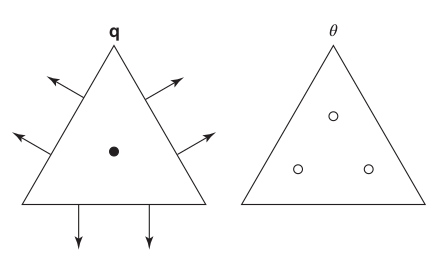
\includegraphics[width=4cm]{images/pair_raviart-thomas/aubb17a}
\end{center}

We now briefly consider the extension of some of the
methods presented in the previous section to quadrilateral
meshes. In this case, we define our approximating spaces
on the reference element $\tilde{K} = [-1,1]^2$ equipped with local
coordinates $(r,s)$. As far as the flux is concerned, the corresponding 
approximation space on each physical element $K$
must be obtained through the use of a suitable transformation
that preserves the normal component of vectorial functions.
This is accomplished by the following (contravariant) Piola's
transformation of vector fields. Suppose that
\[
{\bm F}:\tilde{K} \rightarrow K; 
\qquad
(x,y) = {\bm F}(r,s)
\]
is an invertible map from $\tilde{K}$ onto $K$, with Jacobian matrix
${\bm J}(r,s)$. Given a vector field ${\bm q}(r,s)$ on $\hat{K}$, 
its Piola's transform ${\cal P}({\bm q})(x,y)$ is the vector field on $K$
defined by
\[
{\cal P}({\bm q})(x,y) := \frac{1}{|{\bm J}(r,s)|} {\bm J}(r,s) {\bm q}(r,s)
\qquad 
(x,y)={\bm F}(r,s)
\]
Therefore if
\[
{\bm Q}(\tilde{K})=\text{Span}\{ {\bm q}_i^h; \; i=1,...n_{el}  \}
\]
is an $n_{el}$-dimensional flux approximation space defined on the
reference element $\tilde{K}$, the corresponding space on the physical
element $K$ will be
\[
{\bm Q}(K)=\text{Span}\{{\cal P} ({\bm q}_i^h); \; i=1,...n_{el}  \}
\]
The $RT_{[0]}-P_0$ element. In the reference element $K$, 
we prescribe the approximated flux ${\bm q}^h$  as ($RT_{[0]}$ element)
\[
{\bm q}^h = 
\left\{
\begin{array}{c}
a+br \\ c+ds
\end{array}
\right\}
, \qquad a,b,c\in \R
\]
It is then easily seen from the equation above that the four values
\[
\int_e {\bm q}^h \cdot {\bm n} \; ds 
\qquad \forall e \; \text{edge of} \; \tilde{K}
\]
can be chosen as a set of degrees of freedom. Moreover,
$\text{div} {\bm q}^h$ is constant in $K$,
suggesting the choice of a constant approximated temperature 
$\theta^h$ in $\tilde{K}$ ($P_0$ element). The
degrees of freedom for both ${\bm q}^h$ and $\theta^h$ are shown in
this figure:

\begin{center}
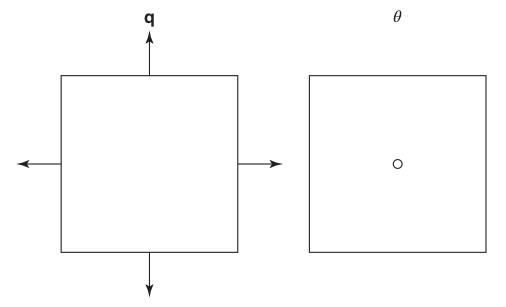
\includegraphics[width=5cm]{images/pair_raviart-thomas/aubb17b}
\end{center}

All the elements presented above have their three-
dimensional counterpart. In this case, the normal component
of the approximated flux ${\bm q}^h$ should not exhibit jumps across
faces of adjacent elements.

In the following figure, we display the tetrahedral version of the
$RT_0-P_0$ element, consisting of a piecewise
constant approximation for the temperature $\theta$ and of the
following element approximating functions for ${\bm q}^h$ (Nedelec,
1980 \cite{nede80}):

\[
{\bm q}^h|_T = {\bm p}_0
+p_0
\left\{\begin{array}{c}
x\\y\\z
\end{array}\right\}
=
\left\{\begin{array}{c}
a_0+p_0x\\ 
b_0+p_0y\\
c_0+p_0z 
\end{array}\right\}
\qquad
a_0,b_0,c_0 \in \R
\]

\begin{center}
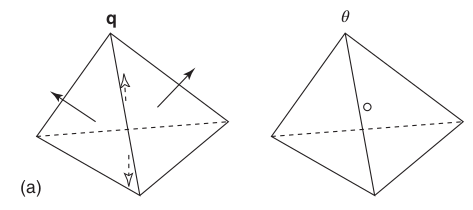
\includegraphics[width=5cm]{images/pair_raviart-thomas/aubb17c}
\end{center}

Therefore, in each tetrahedron $T$, the space for the approximated 
flux has dimension 4 and the degrees of freedom are
precisely the values $\int_f {\bm q}^h\cdot {\bm n}\; d\sigma$ 
on each tetrahedron face $f$.



}
\end{displayquote}


\end{itemize} %global


%......................................................................
\subsection{Degree 1 Raviart–Thomas on a triangle - Lagrange variant}

\url{https://defelement.com/elements/examples/triangle-raviart-thomas-lagrange-1.html}

\begin{center}
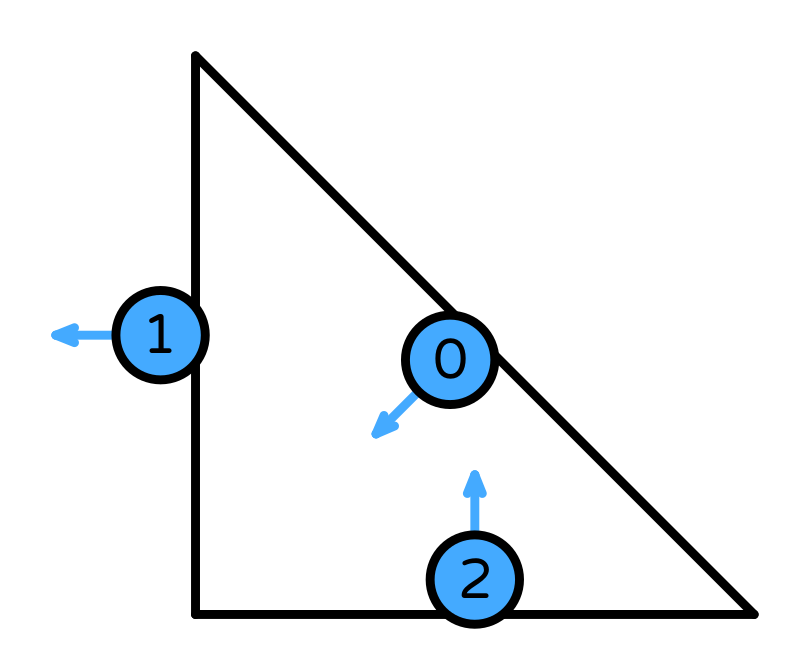
\includegraphics[width=3.3cm]{images/pair_raviart-thomas/element-Raviart-Thomas-variant-equispaced-triangle-1-dofs-large}
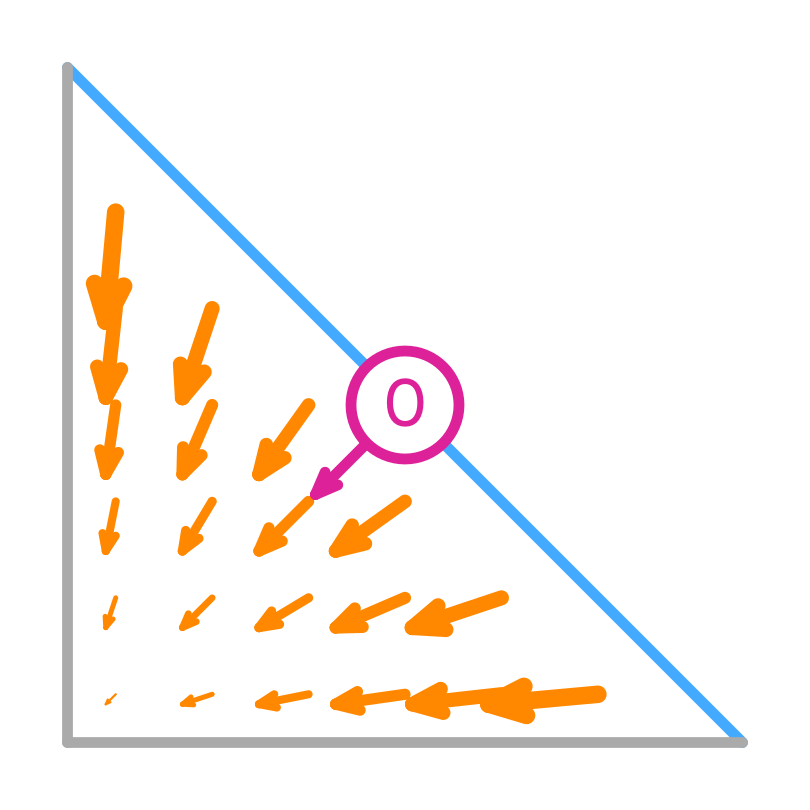
\includegraphics[width=3cm]{images/pair_raviart-thomas/element-Raviart-Thomas-variant-equispaced-triangle-1-0-large}
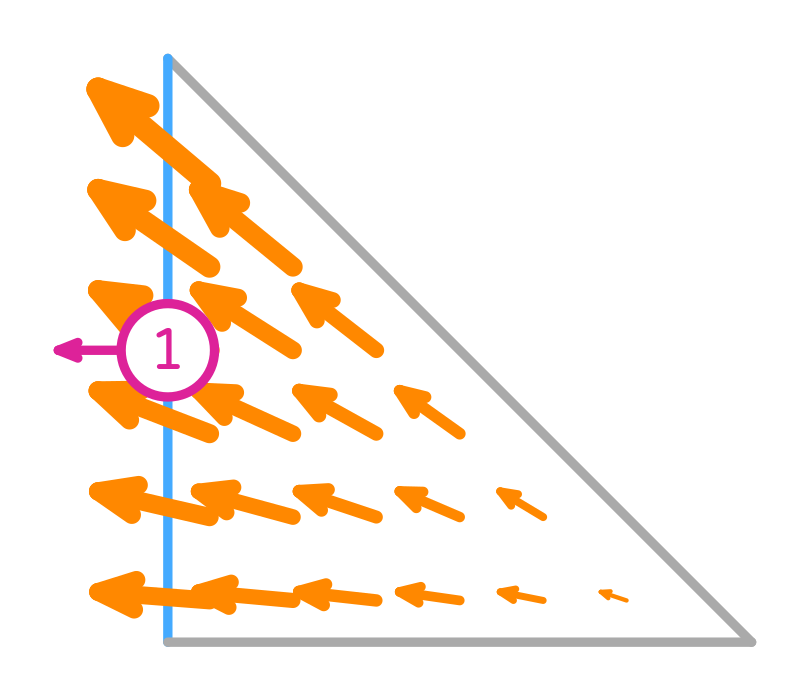
\includegraphics[width=3.3cm]{images/pair_raviart-thomas/element-Raviart-Thomas-variant-equispaced-triangle-1-1-large}
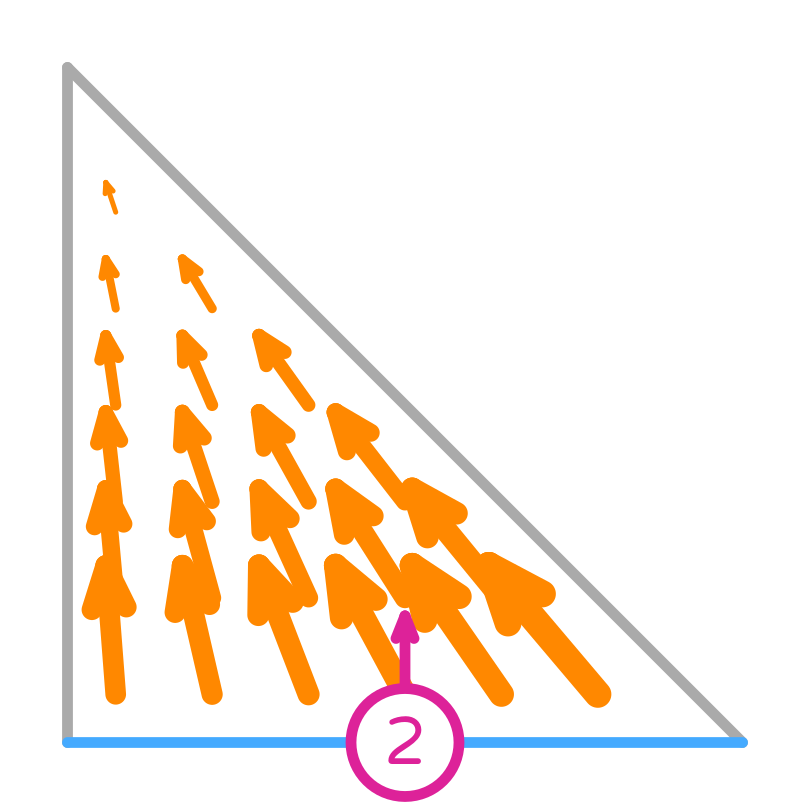
\includegraphics[width=3cm]{images/pair_raviart-thomas/element-Raviart-Thomas-variant-equispaced-triangle-1-2-large}\\
{\captionfont Taken from \url{https://defelement.com/}}
\end{center}

${\cal V}$ is a finite dimensional polynomial space on the element of dimension $3$ and is spanned by \cite{ergu21_72} 
\[
\left( \begin{array}{c} 1 \\ 0  \end{array} \right),
\left( \begin{array}{c} 0 \\ 1  \end{array} \right),
\left( \begin{array}{c} r \\ s  \end{array} \right)
\]
Functionals and basis functions:

\[
l_0: {\bm v} \rightarrow \int_{e_0} {\bm v} \cdot (1) \hat{n}_0
\]
\[
l_1: {\bm v} \rightarrow \int_{e_1} {\bm v} \cdot (1) \hat{n}_1
\]
\[
l_2: {\bm v} \rightarrow \int_{e_2} {\bm v} \cdot (1) \hat{n}_2
\]
where $e_0$ is the 0th edge and $\hat{n}_0$ is the normal to facet 0,
where $e_1$ is the 1st edge and $\hat{n}_1$ is the normal to facet 1,
where $e_2$ is the 2nd edge and $\hat{n}_2$ is the normal to facet 2.

We have then
\[
\vec{\bN}_0(r,s) = \left( \begin{array}{c} -r\\-s  \end{array} \right)
\qquad
\vec{\bN}_1(r,s) = \left( \begin{array}{c} r-1\\s  \end{array} \right)
\qquad
\vec{\bN}_2(r,s) = \left( \begin{array}{c} -r \\ 1-s  \end{array} \right)
\]
These DOFs are associated with edge 0,1,2 of the reference element.

%......................................................................
\subsection{Degree 2 Raviart–Thomas on a triangle - Lagrange variant}

\url{https://defelement.com/elements/examples/triangle-raviart-thomas-lagrange-2.html}

\begin{center}
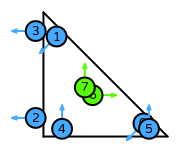
\includegraphics[width=3.3cm]{images/pair_raviart-thomas/element-Raviart-Thomas-variant-equispaced-triangle-2-dofs}
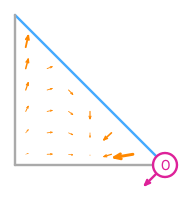
\includegraphics[width=3.3cm]{images/pair_raviart-thomas/element-Raviart-Thomas-variant-equispaced-triangle-2-0}
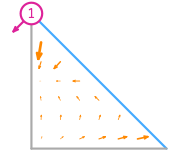
\includegraphics[width=3.3cm]{images/pair_raviart-thomas/element-Raviart-Thomas-variant-equispaced-triangle-2-1}
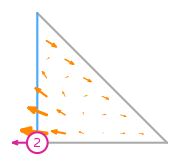
\includegraphics[width=3.3cm]{images/pair_raviart-thomas/element-Raviart-Thomas-variant-equispaced-triangle-2-2}
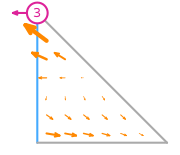
\includegraphics[width=3.3cm]{images/pair_raviart-thomas/element-Raviart-Thomas-variant-equispaced-triangle-2-3}
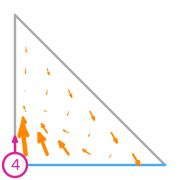
\includegraphics[width=3.3cm]{images/pair_raviart-thomas/element-Raviart-Thomas-variant-equispaced-triangle-2-4}
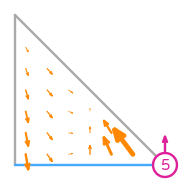
\includegraphics[width=3.3cm]{images/pair_raviart-thomas/element-Raviart-Thomas-variant-equispaced-triangle-2-5}
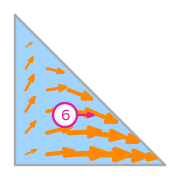
\includegraphics[width=3.3cm]{images/pair_raviart-thomas/element-Raviart-Thomas-variant-equispaced-triangle-2-6}
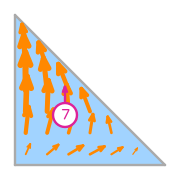
\includegraphics[width=3.3cm]{images/pair_raviart-thomas/element-Raviart-Thomas-variant-equispaced-triangle-2-7}\\
{\captionfont Taken from \url{https://defelement.com/}}
\end{center}


${\cal V}$ is spanned by:
\[
\left( \begin{array}{c} 1 \\ 0  \end{array} \right),
\left( \begin{array}{c} 0 \\ 1  \end{array} \right),
\left( \begin{array}{c} r \\ 0  \end{array} \right),
\left( \begin{array}{c} 0 \\ r  \end{array} \right),
\left( \begin{array}{c} s \\ 0  \end{array} \right),
\left( \begin{array}{c} 0 \\ s  \end{array} \right),
\left( \begin{array}{c} r^2 \\ rs  \end{array} \right),
\left( \begin{array}{c} rs \\ s^2  \end{array} \right)
\]
This basis is also found in \cite{ergu21_72}, example 14.5 (p.163).

We have then
\begin{eqnarray}
\vec{\bN}_0(r,s) &=& \left( \begin{array}{c} 4r(1-2r)\\2s(1-4r)  \end{array} \right) \nn\\
\vec{\bN}_1(r,s) &=& \left( \begin{array}{c} 2r(1-4s)\\4s(1-2s)  \end{array} \right) \nn\\
\vec{\bN}_2(r,s) &=& \left( \begin{array}{c} -8r^2-8rs+12r+6s-4\\2s(-4r-4s+3)  \end{array} \right) \nn\\
\vec{\bN}_3(r,s) &=& \left( \begin{array}{c} 8rs-2r-6s+2\\4s(2s-1)  \end{array} \right) \nn\\
\vec{\bN}_4(r,s) &=& \left( \begin{array}{c} 2r(4r+4s-3)\\8rs-6r+8s^2-12s+4  \end{array} \right) \nn\\
\vec{\bN}_5(r,s) &=& \left( \begin{array}{c} 4r(1-2r)\\-8rs+6r+2s-2  \end{array} \right) \nn\\
\vec{\bN}_6(r,s) &=& \left( \begin{array}{c} 8r(-2r-s+2)\\8s(-2r-s+1)  \end{array} \right) \nn\\
\vec{\bN}_7(r,s) &=& \left( \begin{array}{c} 8r(-r-2s+1)\\8s(-r-2s+2)  \end{array} \right) \nn
\end{eqnarray}
These DOFs are associated with edge 0,1,2 of the reference element.

%......................................................................
\subsection{Degree 1 Raviart–Thomas on a quadrilateral - Lagrange variant}

\begin{center}
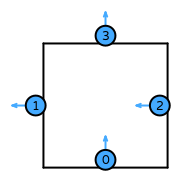
\includegraphics[width=3.5cm]{images/pair_raviart-thomas/element-NCF-variant-equispaced-quadrilateral-1-dofs}
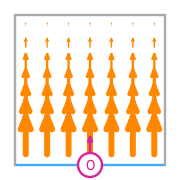
\includegraphics[width=3cm]{images/pair_raviart-thomas/element-NCF-variant-equispaced-quadrilateral-1-0}
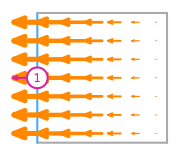
\includegraphics[width=3.5cm]{images/pair_raviart-thomas/element-NCF-variant-equispaced-quadrilateral-1-1}
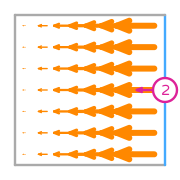
\includegraphics[width=3cm]{images/pair_raviart-thomas/element-NCF-variant-equispaced-quadrilateral-1-2}
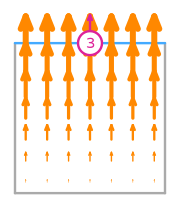
\includegraphics[width=3cm]{images/pair_raviart-thomas/element-NCF-variant-equispaced-quadrilateral-1-3}\\
{\captionfont Taken from \url{https://defelement.com/}}
\end{center}

${\cal V}$ is a finite dimensional polynomial space on the element of dimension $4$ and is spanned by 

\[
\left( \begin{array}{c} 1 \\ 0  \end{array} \right),
\left( \begin{array}{c} 0 \\ 1  \end{array} \right),
\left( \begin{array}{c} r \\ 0  \end{array} \right),
\left( \begin{array}{c} 0 \\ s  \end{array} \right)
\]

Functionals and basis functions:

\[
l_0: {\bm v} \rightarrow \int_{e_0} {\bm v} \cdot (1) \hat{n}_0
\]
\[
l_1: {\bm v} \rightarrow \int_{e_1} {\bm v} \cdot (1) \hat{n}_1
\]
\[
l_2: {\bm v} \rightarrow \int_{e_2} {\bm v} \cdot (1) \hat{n}_2
\]
\[
l_3: {\bm v} \rightarrow \int_{e_3} {\bm v} \cdot (1) \hat{n}_3
\]


where $e_0$ is the 0th edge and $\hat{n}_0$ is the normal to facet 0,
where $e_1$ is the 1st edge and $\hat{n}_1$ is the normal to facet 1,
where $e_2$ is the 2nd edge and $\hat{n}_2$ is the normal to facet 2,
where $e_3$ is the 4th edge and $\hat{n}_3$ is the normal to facet 3.


We have then
\[
\vec{\bN}_0(r,s) = \left( \begin{array}{c} 0 \\ 1-s  \end{array} \right)
\qquad
\vec{\bN}_1(r,s) = \left( \begin{array}{c} r-1 \\0  \end{array} \right)
\qquad
\vec{\bN}_2(r,s) = \left( \begin{array}{c} -r \\ 0  \end{array} \right)
\qquad
\vec{\bN}_3(r,s) = \left( \begin{array}{c} 0 \\s  \end{array} \right)
\]
These DOFs are associated with edge 0,1,2 of the reference element.


%-------------------------------------------------------------------------
\subsection{Degree 1 Raviart–Thomas on a tetrahedron - Lagrange variant}


\begin{center}
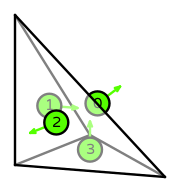
\includegraphics[width=3cm]{images/pair_raviart-thomas/element-Raviart-Thomas-variant-equispaced-tetrahedron-1-dofs}
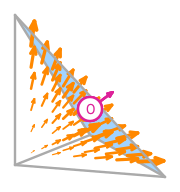
\includegraphics[width=3cm]{images/pair_raviart-thomas/element-Raviart-Thomas-variant-equispaced-tetrahedron-1-0}
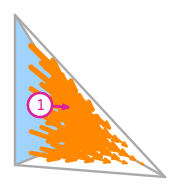
\includegraphics[width=3cm]{images/pair_raviart-thomas/element-Raviart-Thomas-variant-equispaced-tetrahedron-1-1}
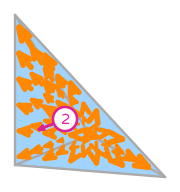
\includegraphics[width=3cm]{images/pair_raviart-thomas/element-Raviart-Thomas-variant-equispaced-tetrahedron-1-2}
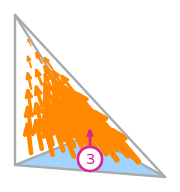
\includegraphics[width=3cm]{images/pair_raviart-thomas/element-Raviart-Thomas-variant-equispaced-tetrahedron-1-3}\\
{\captionfont Taken from \url{https://defelement.com/}}
\end{center}

${\cal V}$ is a finite dimensional polynomial space on the element of dimension $4$ and is spanned by 
\[
\left( \begin{array}{c} 1 \\ 0 \\ 0  \end{array} \right),
\left( \begin{array}{c} 0 \\ 1 \\ 0  \end{array} \right),
\left( \begin{array}{c} 0 \\ 0 \\ 1 \end{array} \right),
\left( \begin{array}{c} r \\ s \\ t \end{array} \right)
\]


\[
\vec{\bN}_0(r,s,t) = \left( \begin{array}{c} 2r \\ 2s \\ 2t  \end{array} \right) 
\quad
\vec{\bN}_1(r,s,t) = \left( \begin{array}{c} 2-2r \\ -2s \\ -2t  \end{array} \right) 
\quad
\vec{\bN}_2(r,s,t) = \left( \begin{array}{c} 2r \\ 2s-2 \\ 2t  \end{array} \right) 
\quad
\vec{\bN}_3(r,s,t) = \left( \begin{array}{c} -2r \\ -2s \\ 2-2t  \end{array} \right) 
\]


%-------------------------------------------------------------------------
\subsection{Degree 1 Raviart–Thomas on a hexahedron - Lagrange variant}

\begin{center}
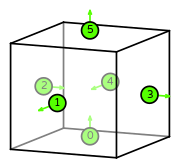
\includegraphics[width=3cm]{images/pair_raviart-thomas/element-NCF-variant-equispaced-hexahedron-1-dofs}
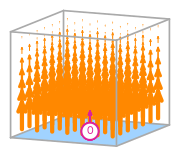
\includegraphics[width=3cm]{images/pair_raviart-thomas/element-NCF-variant-equispaced-hexahedron-1-0}
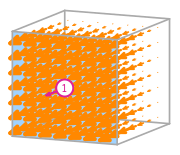
\includegraphics[width=3cm]{images/pair_raviart-thomas/element-NCF-variant-equispaced-hexahedron-1-1}
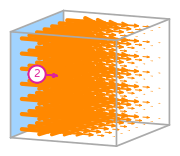
\includegraphics[width=3cm]{images/pair_raviart-thomas/element-NCF-variant-equispaced-hexahedron-1-2}\\
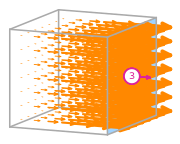
\includegraphics[width=3cm]{images/pair_raviart-thomas/element-NCF-variant-equispaced-hexahedron-1-3}
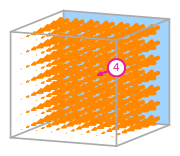
\includegraphics[width=3cm]{images/pair_raviart-thomas/element-NCF-variant-equispaced-hexahedron-1-4}
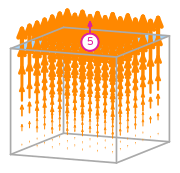
\includegraphics[width=3cm]{images/pair_raviart-thomas/element-NCF-variant-equispaced-hexahedron-1-5}\\
{\captionfont Taken from \url{https://defelement.com/}}
\end{center}


${\cal V}$ is a finite dimensional polynomial space on the element of dimension $6$ and is spanned by 

\[
\left( \begin{array}{c} 1 \\ 0 \\ 0  \end{array} \right),
\left( \begin{array}{c} 0 \\ 1 \\ 0  \end{array} \right),
\left( \begin{array}{c} 0 \\ 0 \\ 1 \end{array} \right),
\left( \begin{array}{c} r \\ 0 \\ 0 \end{array} \right),
\left( \begin{array}{c} 0 \\ s \\ 0 \end{array} \right),
\left( \begin{array}{c} 0 \\ 0 \\ t \end{array} \right).
\]

\[
\vec{\bN}_0(r,s,t) = \left( \begin{array}{c} 0\\0\\1-t  \end{array} \right) 
\quad
\vec{\bN}_1(r,s,t) = \left( \begin{array}{c} 0\\s-1\\0  \end{array} \right) 
\quad
\vec{\bN}_2(r,s,t) = \left( \begin{array}{c} 1-r\\0 \\0  \end{array} \right) 
\]
\[
\vec{\bN}_3(r,s,t) = \left( \begin{array}{c} r\\0\\0  \end{array} \right) 
\quad
\vec{\bN}_4(r,s,t) = \left( \begin{array}{c} 0\\-s\\0  \end{array} \right) 
\quad
\vec{\bN}_5(r,s,t) = \left( \begin{array}{c} 0\\0\\t  \end{array} \right) 
\]



\newpage
What follows is mostly to be found in \textcite{weso19} (2019).

Let us consider a triangulation ${\cal T}_h$ of the domain $\Omega$ 
using triangles or quadrilaterals in 2D and tetrahedrons or
hexahedrons in 3D. For simplicity, edges of elements in 2D will be called as faces, 
and faces in both 2D and 3D will be denoted by $f_j$ . The discrete velocity space is defined as 
\cite{ergu21_72}
\[
{\cal V}_h = \{ \vec{\upnu} | \vec{\upnu}_{|K}  \in RT_0(K) , K\in {\cal T}_h \text{ and } \vec\in {\cal V} \}
\]
with ${\cal V} \subset H(\text{div},\Omega)$ and
where $RT_0$ is the lowest-order Raviart-Thomas space on the element $K$. 
Let the basis (shape) functions for the velocity and pressure spaces be denoted $\bN^\upnu_i$ and 
$\bN^p_j$, respectively. The pressures are approximated by piecewise
constant basis functions, and we denote by ${\cal Q}_h$ the discrete pressure space. For the velocity degrees of freedom we
consider the average values of the normal components over the element faces. Specifically, the velocity degrees of
freedom are defined as
\begin{equation}
\frac{1}{|f_j|} \int_{f_j} \vec{\bN}^\upnu_i( \vec{x}_j) \cdot \vec{n}_j \; dl = \delta_{ij} 
\label{eq:RTbfdef}
\end{equation}
where $\delta_{ij}$ is the Kronecker delta, $\vec{n}_j$ is the unit outward normal of face $j$ 
and $\vec{x}_j$ is its coordinate. In the calculations
of the basis functions below, we use centers of the corresponding faces.

%----------------------------
\subsection{Triangle, RT0}

\begin{center}
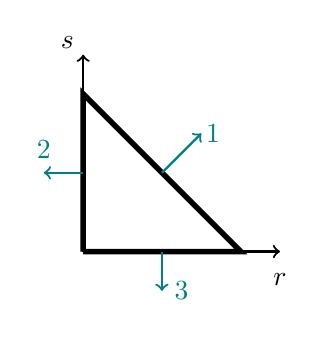
\begin{tikzpicture}
%\draw[step=0.5cm,gray,very thin] (0,0) grid (4.5,4.5); %background grid
\draw [thick,->] (1,1) -- (3.5,1);
\draw [thick,->] (1,1) -- (1,3.5);
\node[] at (3.5,0.65) {$r$};
\node[] at (0.8,3.65) {$s$};
\draw[line width=.7mm] (1,1) -- (3,1) -- (1,3) -- (1,1);   
\draw [thick,teal,->] (2,2) -- (2.5,2.5);
\draw [thick,teal,->] (2,1) -- (2,0.5);
\draw [thick,teal,->] (1,2) -- (0.5,2);
\node[teal] at (2.65,2.5) {$1$};
\node[teal] at (2.25,0.5) {$3$};
\node[teal] at (0.5,2.3) {$2$};
\end{tikzpicture}
\end{center}


The basis functions in the reference triangle are defined as (see John reference earlier)
\[
\vec{\bN}_i(r,s)
=\vec{a} + b  \left(\begin{array}{c} r\\s \end{array}\right)
=\left(\begin{array}{c} a_1+b r \\ a_2 + b s \end{array}\right)
\qquad i=1,2,3
\]

\begin{itemize}
\item face $j=1$. 
Using Eq.~\eqref{eq:RTbfdef} we can write for the first face (the middle of this face has coordinates 
$\vec{x}_1=(1/2,1/2)$, the normal is $\vec{n}_1=(1/\sqrt2,1/\sqrt2)$ and $|f_1|=\sqrt 2$):
\begin{eqnarray}
\delta_{i1}=
\frac{1}{|f_1|} \int_{f_1} \vec{\bN}^\upnu_i( \vec{x}_1) \cdot \vec{n}_1 \; dl
&=& \frac{1}{\sqrt 2} \int_{f_1} \vec{\bN}^\upnu_i( 1/2,1/2) \cdot 
\left(\begin{array}{c} 1/\sqrt2 \\1/\sqrt2 \end{array}\right) \; dl \nn\\
&=& \frac{1}{\sqrt 2} \int_{f_1} 
\left(\begin{array}{c} a_1+b\cdot 1/2 \\ a_2 + b \cdot 1/2 \end{array}\right)
\cdot 
\left(\begin{array}{c} 1/\sqrt2 \\1/\sqrt2 \end{array}\right) \; dl \nn\\
&=& \frac{1}{\sqrt 2} \frac{1}{\sqrt2} (a_1 + a_2+b) \int_{f_1} 1 \; dl \nn\\
&=& \frac{1}{\sqrt 2} \frac{1}{\sqrt2} (a_1 + a_2+b) \sqrt 2 \nn\\
&=& \frac{1}{\sqrt 2}  (a_1 + a_2+b) \label{eq:RT0tri1}
\end{eqnarray}


\item face $j=2$.
Using Eq.~\eqref{eq:RTbfdef} we can write for the second face (the middle of this face has coordinates $\vec{x}_2=(0,1/2)$, the normal is $\vec{n}_2=(-1,0)$ and $|f_2|=1$):

\begin{eqnarray}
\delta_{i2}=
\frac{1}{|f_2|} \int_{f_2} \vec{\bN}^\upnu_i( \vec{x}_2) \cdot \vec{n}_2 \; dl
&=& 
 \int_{0}^1  \vec{\bN}^\upnu_i( 0,1/2) \cdot 
\left(\begin{array}{c} -1 \\0 \end{array}\right) \; ds \nn\\
&=&  \int_{0}^1 
\left(\begin{array}{c} a_1 + b \cdot 0 \\ a_2 + b \cdot 1/2 \end{array}\right)
\cdot 
\left(\begin{array}{c} -1 \\ 0 \end{array}\right) \; ds \nn\\
&=& -   a_1 \int_0^1 ds \nn\\
&=& -   a_1 \label{eq:RT0tri2}
\end{eqnarray}


\item face $j=3$
Using Eq.~\eqref{eq:RTbfdef} we can write for the third face (the middle of this face has coordinates 
$\vec{x}_3=(1/2,0)$, the normal is $\vec{n}_3=(0,-1)$  and $|f_3|=1$):

\begin{eqnarray}
\delta_{i3}=
\frac{1}{|f_3|} \int_{f_3} \vec{\bN}^\upnu_i( \vec{x}_3) \cdot \vec{n}_3 \; dl
&=& 
 \int_{0}^{1} \vec{\bN}^\upnu_i( 1/2,0) \cdot \left(\begin{array}{c} 0 \\-1 \end{array}\right) \; dr \nn\\
&=&
 \int_{0}^{1} \left(\begin{array}{c} a_1+b\cdot 1/2 \\ a_2 + b \cdot 0 \end{array}\right) \cdot \left(\begin{array}{c} 0 \\ -1 \end{array}\right) \; dr \nn\\
&=& -  a_2 \int_{0}^{1}  dr \nn\\
&=& - a_2  \label{eq:RT0tri3}
\end{eqnarray}
\end{itemize}

We can now compute the three basis functions: 

\begin{itemize}
\item Case $i=1$: Using Eqs.~\eqref{eq:RT0tri1},\eqref{eq:RT0tri2},\eqref{eq:RT0tri3} we can write

\begin{eqnarray}
\frac{1}{\sqrt 2}  (a_1 + a_2+b)  &=&  1 \nn\\
-a_1 &=& 0 \nn\\
-a_2 &=& 0 \nn
\end{eqnarray}
which yields $a_1=a_2=0$ and $b=\sqrt 2$, i.e.
\[
\vec{\bN}^\upnu_1 (r,s) = \sqrt 2
\left(
\begin{array}{c}
r \\ s
\end{array}
\right)
\]

\item Case $i=2$: Using Eqs.~\eqref{eq:RT0tri1},\eqref{eq:RT0tri2},\eqref{eq:RT0tri3} we can write
\begin{eqnarray}
\frac{1}{\sqrt 2}  (a_1 + a_2+b)  &=&  0 \nn\\
-a_1 &=& 1 \nn\\
-a_2 &=& 0 \nn
\end{eqnarray}
which yields $a_1=-1$, $a_2=0$ and $b=-a_1=1$, i.e.
\[
\vec{\bN}^\upnu_2 (r,s) =
\left(
\begin{array}{c}
-1 +r \\ s
\end{array}
\right)
\]


\item Case $i=3$: Using Eqs.~\eqref{eq:RT0tri1},\eqref{eq:RT0tri2},\eqref{eq:RT0tri3} we can write
\begin{eqnarray}
\frac{1}{\sqrt 2}  (a_1 + a_2+b)  &=&  0 \nn\\
-a_1 &=& 0 \nn\\
-a_2 &=& 1 \nn
\end{eqnarray}
which yields $a_1=0$, $a_2=-1$ and $b=-a_2=1$, i.e.
\[
\vec{\bN}^\upnu_3 (r,s) =
\left(
\begin{array}{c}
 r \\ -1 +  s
\end{array}
\right)
\]

\end{itemize}


In the end:
\begin{mdframed}[backgroundcolor=blue!5]
\[
\vec{\bN}^\upnu_1 (r,s) = \sqrt 2
\left(
\begin{array}{c}
r \\ s
\end{array}
\right)
\qquad
\vec{\bN}^\upnu_2 (r,s) =
\left(
\begin{array}{c}
-1 +r \\ s
\end{array}
\right)
\qquad
\vec{\bN}^\upnu_3 (r,s) =
\left(
\begin{array}{c}
 r \\ -1 +  s
\end{array}
\right)
\]
\end{mdframed}


%----------------------------
\subsection{Quadrilateral, RT0}


\begin{center}
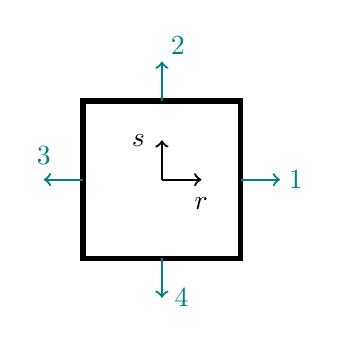
\begin{tikzpicture}
%\draw[step=0.5cm,gray,very thin] (0,0) grid (4.5,4.5); %background grid
\draw [thick,->] (2,2) -- (2.5,2);
\draw [thick,->] (2,2) -- (2,2.5);
\node[] at (2.5,1.7) {$r$};
\node[] at (1.7,2.5) {$s$};
\draw[line width=.7mm] (1,1) -- (3,1) -- (3,3) -- (1,3) --cycle;   
\draw [thick,teal,->] (3,2) -- (3.5,2);
\draw [thick,teal,->] (2,3) -- (2,3.5);
\draw [thick,teal,->] (2,1) -- (2,0.5);
\draw [thick,teal,->] (1,2) -- (0.5,2);
\node[teal] at (3.7,2) {$1$};
\node[teal] at (2.2,3.7) {$2$};
\node[teal] at (0.5,2.3) {$3$};
\node[teal] at (2.25,0.5) {$4$};
\end{tikzpicture}
\end{center}

The basis functions are defined as (see literature section earlier on) 
\[
\vec{\bN}_i(r,s)
=\vec{a} + b  \left(\begin{array}{c} r\\s \end{array}\right)
=\left(\begin{array}{c} a_1+b_1 r \\ a_2 + b_2 s \end{array}\right)
\qquad i=1,2,3,4
\]
In this case all faces have the same length, i.e. $|f_j|=2$.

\begin{itemize}
\item face $j=1$. We can write for the first face (the middle of this face has coordinates 
$\vec{x}_1=(1,0)$, the normal is $\vec{n}_1=(1,0)$):

\begin{eqnarray}
\delta_{i1}=
\frac{1}{|f_1|} \int_{f_1}
\vec{\bN}^\upnu_i( \vec{x}_1) \cdot \vec{n}_1 \; dl
&=&\frac12  \int_{f_1} \vec{\bN}^\upnu_i( 1,0) \cdot 
\left(\begin{array}{c} 1 \\ 0 \end{array}\right) \; dl \nn\\
&=& \frac12\int_{f_1} 
\left(\begin{array}{c} a_1+b_1\cdot 1 \\ a_2 + b_2 \cdot 0 \end{array}\right)
\cdot \left(\begin{array}{c} 1 \\ 0 \end{array}\right) \; dl \nn\\
&=& \frac12 \int_{-1}^{+1} (a_1+b_1) ds \nn\\
&=& a_1+b_1
\end{eqnarray}



\item face $j=2$. We can write for the first face (the middle of this face has coordinates 
$\vec{x}_2=(0,1)$, the normal is $\vec{n}_2=(0,1)$):

\begin{eqnarray}
\delta_{i2}=
\frac{1}{|f_2|} \int_{f_2}
\vec{\bN}^\upnu_i( \vec{x}_2) \cdot \vec{n}_2 \; dl
&=&\frac12  \int_{f_1} \vec{\bN}^\upnu_i( 0,1) \cdot 
\left(\begin{array}{c} 0 \\ 1 \end{array}\right) \; dl \nn\\
&=& \frac12\int_{f_1} 
\left(\begin{array}{c} a_1+b_1\cdot 0 \\ a_2 + b_2 \cdot 1 \end{array}\right)
\cdot \left(\begin{array}{c} 0 \\ 1 \end{array}\right) \; dl \nn\\
&=& \frac12 \int_{-1}^{+1} (a_2+b_2) dr \nn\\
&=& a_2+b_2
\end{eqnarray}


\item face $j=3$. We can write for the first face (the middle of this face has coordinates 
$\vec{x}_3=(-1,0)$, the normal is $\vec{n}_3=(-1,0)$):


\begin{eqnarray}
\delta_{i3}=
\frac{1}{|f_3|} \int_{f_3}
\vec{\bN}^\upnu_i( \vec{x}_3) \cdot \vec{n}_3 \; dl
&=&\frac12  \int_{f_1} \vec{\bN}^\upnu_i( -1,0) \cdot 
\left(\begin{array}{c} -1 \\ 0 \end{array}\right) \; dl \nn\\
&=& \frac12\int_{f_1} 
\left(\begin{array}{c} a_1+b_1\cdot -1 \\ a_2 + b_2 \cdot 0 \end{array}\right)
\cdot \left(\begin{array}{c} -1 \\ 0 \end{array}\right) \; dl \nn\\
&=& -\frac12 \int_{-1}^{+1} (a_1-b_1) ds \nn\\
&=& -a_1+b_1
\end{eqnarray}




\item face $j=4$. We can write for the first face (the middle of this face has coordinates 
$\vec{x}_4=(0,-1)$, the normal is $\vec{n}_4=(0,-1)$):
\end{itemize}

\begin{eqnarray}
\delta_{i4}=
\frac{1}{|f_4|} \int_{f_4}
\vec{\bN}^\upnu_i( \vec{x}_4) \cdot \vec{n}_4 \; dl
&=&\frac12  \int_{f_1} \vec{\bN}^\upnu_i( 0,-1) \cdot 
\left(\begin{array}{c} 0 \\ -1 \end{array}\right) \; dl \nn\\
&=& \frac12\int_{f_1} 
\left(\begin{array}{c} a_1+b_1\cdot 0 \\ a_2 + b_2 \cdot -1 \end{array}\right)
\cdot \left(\begin{array}{c} 0 \\ -1 \end{array}\right) \; dl \nn\\
&=& -\frac12 \int_{-1}^{+1} (a_2-b_2) dr \nn\\
&=& -a_2+b_2
\end{eqnarray}



\begin{itemize}
\item Case $i=1$. We have to solve
\[
\left(\begin{array}{cccc}
1 & 0 & 1 & 0 \\
0 & 1 & 0 & 1 \\
-1 & 0 & 1 & 0\\
0 & -1 & 0 & 1
\end{array}\right)
\cdot
\left(\begin{array}{c}
a_1 \\ a_2 \\ b_1 \\ b_2
\end{array}\right)
=
\left(\begin{array}{c}
1 \\ 0 \\ 0 \\ 0
\end{array}\right)
\]
which yields
$a_1=1/2$, $b_1=1/2$, $a_2=b_2=0$.


\item Case $i=2$. We have to solve
\[
\left(\begin{array}{cccc}
1 & 0 & 1 & 0 \\
0 & 1 & 0 & 1 \\
-1 & 0 & 1 & 0\\
0 & -1 & 0 & 1
\end{array}\right)
\cdot
\left(\begin{array}{c}
a_1 \\ a_2 \\ b_1 \\ b_2
\end{array}\right)
=
\left(\begin{array}{c}
0 \\ 1 \\ 0 \\ 0
\end{array}\right)
\]
which yields $a_1=0$, $b_1=0$, $a_2=1/2$, $b_2=1/2$.


\item Case $i=3$. We have to solve
\[
\left(\begin{array}{cccc}
1 & 0 & 1 & 0 \\
0 & 1 & 0 & 1 \\
-1 & 0 & 1 & 0\\
0 & -1 & 0 & 1
\end{array}\right)
\cdot
\left(\begin{array}{c}
a_1 \\ a_2 \\ b_1 \\ b_2
\end{array}\right)
=
\left(\begin{array}{c}
0 \\ 0 \\ 1 \\ 0
\end{array}\right)
\]
which $a_1=-1/2$, $b_1=1/2$, $a_2=0$, $b_2=0$.

\item Case $i=4$. We have to solve
\[
\left(\begin{array}{cccc}
1 & 0 & 1 & 0 \\
0 & 1 & 0 & 1 \\
-1 & 0 & 1 & 0\\
0 & -1 & 0 & 1
\end{array}\right)
\cdot
\left(\begin{array}{c}
a_1 \\ a_2 \\ b_1 \\ b_2
\end{array}\right)
=
\left(\begin{array}{c}
0 \\ 0 \\ 0 \\ 1
\end{array}\right)
\]
which yields 
$a_1=0$, $b_1=0$, $a_2=-1/2$, $b_2=1/2$.

\end{itemize}

In the end we arrive at the following basis functions:

\begin{mdframed}[backgroundcolor=blue!5]
\begin{eqnarray}
\vec{\bN}^\upnu_1 (r,s) &=& 
\left(\begin{array}{c} \frac12 (1+r) \\ 0 \end{array}\right) \nn\\
\vec{\bN}^\upnu_2 (r,s) &=& 
\left(\begin{array}{c} 0 \\ \frac12 (1+s)  \end{array}\right) \nn\\
\vec{\bN}^\upnu_3 (r,s) &=& 
\left(\begin{array}{c} \frac12 (-1+r) \\ 0 \end{array}\right) \nn\\
\vec{\bN}^\upnu_4 (r,s) &=& 
\left(\begin{array}{c} 0 \\ \frac12 (-1+s)  \end{array}\right)
\end{eqnarray}
\end{mdframed}



%-------------------------------
\subsection{Tetrahedron, RT0}

The basis functions in the reference triangle are defined as (see literature section 
earlier on)
\[
\vec{\bN}_i(r,s,t)
=\vec{a} + b  \left(\begin{array}{c} r\\s\\t \end{array}\right)
=\left(\begin{array}{c} a_1+b r \\ a_2 + b s \\ a_3 + b t \end{array}\right)
\qquad i=1,2,3,4
\]

\begin{center}
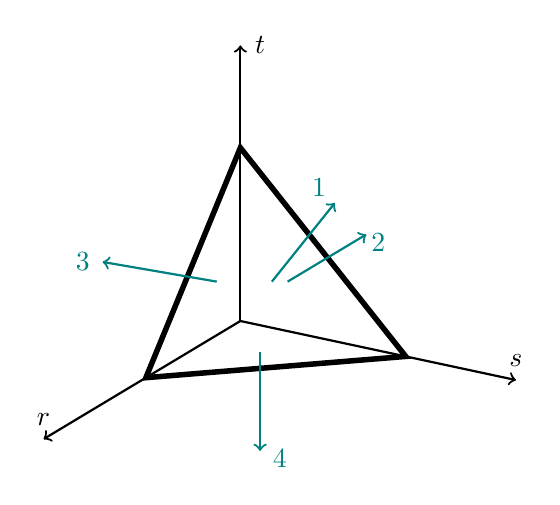
\begin{tikzpicture}
%\draw[step=0.5cm,gray,very thin] (0,0) grid (7,6); %background grid
\draw [thick,->] (3,2) -- (0.5,0.5);
\draw [thick,->] (3,2) -- (6.5,1.25);
\draw [thick,->] (3,2) -- (3,5.5);
\node[] at (0.5,0.75) {$r$};
\node[] at (6.5,1.5) {$s$};
\node[] at (3.25,5.5) {$t$};
\draw[line width=.7mm] (1.8,1.28) -- (5.1,1.55) -- (3,4.2)  --cycle;   
\draw [thick,teal,->] (2.7,2.5) -- (1.25,2.75); \node[teal] at (1,2.75) {$3$};
\draw [thick,teal,->] (3.6,2.5) -- (4.6,3.1); \node[teal] at (4.75,3) {$2$};
\draw [thick,teal,->] (3.4,2.5) -- (4.2,3.5); \node[teal] at (4,3.7) {$1$};
\draw [thick,teal,->] (3.25,1.6) -- (3.25,0.35); \node[teal] at (3.5,0.25) {$4$};
\end{tikzpicture}
\end{center}



\begin{itemize}
\item face $j=1$. We can write for the first face (the middle of this face has coordinates 
$\vec{x}_1=(1/3,1/3,1/3)$, the normal is $\vec{n}_1=\frac{1}{\sqrt3}(1,1,1)$):

\begin{eqnarray}
\delta_{i1}=
\frac{1}{|f_1|} \iint_{f_1}
\vec{\bN}^\upnu_i( \vec{x}_1) \cdot \vec{n}_1 \; dS
&=&\frac{1}{|f_1|} \iint_{f_1} \vec{\bN}^\upnu_i( 1/3,1/3,1/3) \cdot 
\frac{1}{\sqrt3}\left(\begin{array}{c} 1 \\ 1 \\1 \end{array}\right) \; dS \nn\\
&=& \frac{1}{|f_1|} \iint_{f_1} 
\left(\begin{array}{c} a_1+b\cdot 1/3 \\ a_2 + b \cdot 1/3 \\ a_3 + b \cdot 1/3 \end{array}\right)
\cdot \frac{1}{\sqrt3} \left(\begin{array}{c} 1 \\ 1 \\ 1 \end{array}\right) \; dS \nn\\
&=& \frac{1}{|f_1|} \iint_{f_1} (a_1+a_2+a_3 + b) dS \nn\\
&=& \frac{1}{\sqrt 3} (a_1+a_2+a_3+b)
\end{eqnarray}

\item face $j=2$. We can write for the first face (the middle of this face has coordinates 
$\vec{x}_1=(0,1/3,1/3)$, the normal is $\vec{n}_1=(-1,0,0)$):

\begin{eqnarray}
\delta_{i2}=
\frac{1}{|f_2|} \iint_{f_2}
\vec{\bN}^\upnu_i( \vec{x}_1) \cdot \vec{n}_1 \; dS
&=&\frac{1}{|f_2|} \iint_{f_2} \vec{\bN}^\upnu_i( 0,1/3,1/3) \cdot 
\left(\begin{array}{c} -1\\0\\0 \end{array}\right) \; dS \nn\\
&=& \frac{1}{|f_2|} \iint_{f_2} 
\left(\begin{array}{c} a_1+b\cdot 0 \\ a_2 + b \cdot 1/3 \\ a_3 + b \cdot 1/3 \end{array}\right)
\cdot  \left(\begin{array}{c} -1\\0\\0 \end{array}\right) \; dS \nn\\
&=& \frac{1}{|f_2|} \iint_{f_2} (-a_1) dS \nn\\
&=& -a_1
\end{eqnarray}

\item face $j=3$. We can write for the first face (the middle of this face has coordinates 
$\vec{x}_1=(1/3,0,1/3)$, the normal is $\vec{n}_1=(0,-1,0)$):

\begin{eqnarray}
\delta_{i3}=
\frac{1}{|f_3|} \iint_{f_3}
\vec{\bN}^\upnu_i( \vec{x}_1) \cdot \vec{n}_1 \; dS
&=&\frac{1}{|f_3|} \iint_{f_3} \vec{\bN}^\upnu_i( 1/3,0,1/3) \cdot 
\left(\begin{array}{c} 0\\-1\\0 \end{array}\right) \; dS \nn\\
&=& \frac{1}{|f_3|} \iint_{f_3} 
\left(\begin{array}{c} a_1+b\cdot 1/3 \\ a_2 + b \cdot 0 \\ a_3 + b \cdot 1/3 \end{array}\right)
\cdot  \left(\begin{array}{c} 0\\-1\\0 \end{array}\right) \; dS \nn\\
&=& \frac{1}{|f_3|} \iint_{f_3} (-a_2) dS \nn\\
&=& -a_2
\end{eqnarray}



\item face $j=4$. We can write for the first face (the middle of this face has coordinates 
$\vec{x}_1=(1/3,1/3,0)$, the normal is $\vec{n}_1=(0,0,-1)$):

\begin{eqnarray}
\delta_{i4}=
\frac{1}{|f_4|} \iint_{f_4}
\vec{\bN}^\upnu_i( \vec{x}_1) \cdot \vec{n}_1 \; dS
&=&\frac{1}{|f_4|} \iint_{f_4} \vec{\bN}^\upnu_i( 1/3,1/3,0) \cdot 
\left(\begin{array}{c} 0\\0\\-1 \end{array}\right) \; dS \nn\\
&=& \frac{1}{|f_4|} \iint_{f_4} 
\left(\begin{array}{c} a_1+b\cdot 1/3 \\ a_2 + b \cdot 1/3 \\ a_3 + b \cdot  0\end{array}\right)
\cdot  \left(\begin{array}{c} 0\\0\\-1 \end{array}\right) \; dS \nn\\
&=& \frac{1}{|f_4|} \iint_{f_4} (-a_3) dS \nn\\
&=& -a_3
\end{eqnarray}

\end{itemize}



\begin{itemize}
\item Case $i=1$. We have to solve
\[
\left(\begin{array}{cccc}
1/\sqrt3 & 1/\sqrt3 & 1/\sqrt3 & 1/\sqrt3 \\
-1 & 0 & 0 & 0 \\
0 & -1 & 0 & 0 \\
0 & 0 & -1 & 0
\end{array}\right)
\cdot
\left(\begin{array}{c}
a_1 \\ a_2 \\ a_3 \\ b
\end{array}\right)
=
\left(\begin{array}{c}
1 \\ 0 \\ 0 \\ 0
\end{array}\right)
\]
which yields $a_1=a_2=a_3=0$ and $b=1/\sqrt3$.

\item Case $i=2$. We have to solve
\[
\left(\begin{array}{cccc}
1/\sqrt3 & 1/\sqrt3 & 1/\sqrt3 & 1/\sqrt3 \\
-1 & 0 & 0 & 0 \\
0 & -1 & 0 & 0 \\
0 & 0 & -1 & 0
\end{array}\right)
\cdot
\left(\begin{array}{c}
a_1 \\ a_2 \\ a_3 \\ b
\end{array}\right)
=
\left(\begin{array}{c}
0 \\ 1 \\ 0 \\ 0
\end{array}\right)
\]

which yields $a_2=a_3=0$, $a_1=-1$ and $b=-a_1=1$.

\item Case $i=3$. We have to solve
\[
\left(\begin{array}{cccc}
1/\sqrt3 & 1/\sqrt3 & 1/\sqrt3 & 1/\sqrt3 \\
-1 & 0 & 0 & 0 \\
0 & -1 & 0 & 0 \\
0 & 0 & -1 & 0
\end{array}\right)
\cdot
\left(\begin{array}{c}
a_1 \\ a_2 \\ a_3 \\ b
\end{array}\right)
=
\left(\begin{array}{c}
0 \\ 0 \\ 1 \\ 0
\end{array}\right)
\]
which yields $a_1=a_3=0$, $a_2=-1$ and $b=-a_2=1$.

\item Case $i=4$. We have to solve
\[
\left(\begin{array}{cccc}
1/\sqrt3 & 1/\sqrt3 & 1/\sqrt3 & 1/\sqrt3 \\
-1 & 0 & 0 & 0 \\
0 & -1 & 0 & 0 \\
0 & 0 & -1 & 0
\end{array}\right)
\cdot
\left(\begin{array}{c}
a_1 \\ a_2 \\ a_3 \\ b
\end{array}\right)
=
\left(\begin{array}{c}
0 \\ 0 \\ 0 \\ 1
\end{array}\right)
\]
which yields $a_1=a_2=0$, $a_3=-1$ and $b=-a_3=1$.

\end{itemize}

In the end

\begin{mdframed}[backgroundcolor=blue!5]
\begin{eqnarray}
\vec{\bN}^\upnu_1 (r,s) &=& \frac{1}{\sqrt3}
\left(\begin{array}{c} r \\s \\ t \end{array}\right) \nn\\
\vec{\bN}^\upnu_2 (r,s) &=& 
\left(\begin{array}{c} -1+r \\ s \\t\end{array}\right) \nn\\
\vec{\bN}^\upnu_3 (r,s) &=& 
\left(\begin{array}{c} r \\ -1+s \\t \end{array}\right) \nn\\
\vec{\bN}^\upnu_4 (r,s) &=& 
\left(\begin{array}{c} r\\s\\-1+t \end{array}\right)
\end{eqnarray}
\end{mdframed}

%--------------------------------
\subsection{Hexahedron, RT0}

The basis functions in the reference triangle are defined as (see literature section earlier on) 
\[
\vec{\bN}_i(r,s,t)
=\vec{a} + b  \left(\begin{array}{c} r\\s\\t \end{array}\right)
=\left(\begin{array}{c} a_1+b_1 r \\ a_2 + b_2 s \\ a_3 + b_3 t \end{array}\right)
\qquad i=1,2,3,4,5,6
\]

\begin{center}
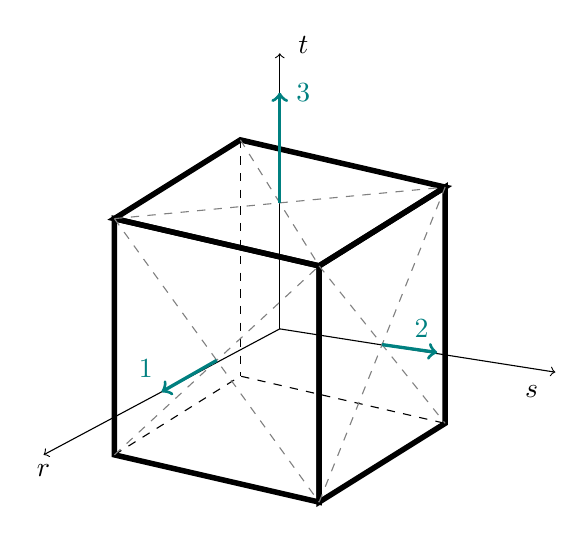
\begin{tikzpicture}
%\draw[step=0.5cm,gray,very thin] (0,0) grid (8,7); %background grid

\draw [thin,->] (4,3) -- (1,1.4); % r
\draw [thin,->] (4,3) -- (7.5,2.45); % s
\draw [thin,->] (4,3) -- (4,6.5); % t

\node[] at (1,1.2) {$r$};
\node[] at (7.2,2.2) {$s$};
\node[] at (4.3,6.6) {$t$};
\draw[line width=.7mm] (4.5,0.8) -- (6.1,1.8) -- (6.1,4.8) --(4.5,3.8) --cycle; %face 2  
\draw[line width=.7mm] (4.5,0.8) -- (4.5,3.8) -- (1.9,4.4) --(1.9,1.4) --cycle;  % face 1
\draw[line width=.7mm] (1.9,4.4) -- (4.5,3.8) -- (6.1,4.8) --(3.5,5.4) --cycle;

\draw[dashed] (1.9,1.4)--(3.5,2.4) -- (6.1,1.8);
\draw[dashed] (3.5,5.4)--(3.5,2.4) ;

\draw[dashed,gray] (4.5,0.8)--(6.1,4.8) ; %face 2
\draw[dashed,gray] (4.5,3.8)--(6.1,1.8) ; %face 2

\draw[dashed,gray] (1.9,4.4)--(6.1,4.8) ; %face 3
\draw[dashed,gray] (3.5,5.4)--(4.5,3.8) ; %face 3

\draw[dashed,gray] (1.9,1.4)--(4.5,3.8); %face 1
\draw[dashed,gray] (1.9,4.4)--(4.5,0.8); % face1


\draw [very thick,teal,->] (3.2,2.6) -- (2.5,2.2); \node[teal] at (2.3,2.5) {$1$};
\draw [very thick,teal,->] (5.3,2.8) -- (6,2.7); \node[teal] at (5.8,3) {$2$};
\draw [very thick,teal,->] (4,4.6) -- (4,6); \node[teal] at (4.3,6) {$3$};

\end{tikzpicture}
\end{center}


In this case all faces have the same length, i.e. $|f_j|=4$.

\begin{itemize}
\item face $j=1$. We can write for the first face (the middle of this face has coordinates 
$\vec{x}_1=(1,0,0)$, the normal is $\vec{n}_1=(1,0,0)$):


\begin{eqnarray}
\delta_{i1}=
\frac{1}{|f_1|} \iint_{f_1}
\vec{\bN}^\upnu_i( \vec{x}_1) \cdot \vec{n}_1 \; dS
&=&\frac{1}{|f_1|} \iint_{f_1} \vec{\bN}^\upnu_i( 1,0,0) \cdot 
\left(\begin{array}{c} 1 \\ 0  \\ 0\end{array}\right) \; dS \nn\\
&=& \frac{1}{|f_1|} \iint_{f_1} 
\left(\begin{array}{c} a_1+b_1\cdot 1 \\ a_2 + b_2 \cdot 0 \\ a_3 + b_3\cdot 0 \end{array}\right)
\cdot \left(\begin{array}{c} 1 \\ 0 \\ 0 \end{array}\right) \; dS \nn\\
&=& \frac{1}{|f_1|} \iint_{f_1} (a_1+b_1) dS \nn\\
&=& a_1+b_1
\end{eqnarray}


\item face $j=2$. We can write for the first face (the middle of this face has coordinates 
$\vec{x}_2=(0,1,0)$, the normal is $\vec{n}_2=(0,1,0)$):

\begin{eqnarray}
\delta_{i2}=
\frac{1}{|f_2|} \iint_{f_2}
\vec{\bN}^\upnu_i( \vec{x}_2) \cdot \vec{n}_2 \; dS
&=&\frac{1}{|f_2|} \iint_{f_2} \vec{\bN}^\upnu_i( 0,1,0) \cdot 
\left(\begin{array}{c} 0 \\ 1  \\ 0\end{array}\right) \; dS \nn\\
&=& \frac{1}{|f_2|} \iint_{f_2} 
\left(\begin{array}{c} a_1+b_1\cdot 0 \\ a_2 + b_2 \cdot 1 \\ a_3 + b_3\cdot 0 \end{array}\right)
\cdot \left(\begin{array}{c} 0 \\ 1 \\ 0 \end{array}\right) \; dS \nn\\
&=& \frac{1}{|f_2|} \iint_{f_2} (a_2+b_2) dS \nn\\
&=& a_2+b_2
\end{eqnarray}


\item face $j=3$. We can write for the first face (the middle of this face has coordinates 
$\vec{x}_3=(0,0,1)$, the normal is $\vec{n}_3=(0,0,1)$):


\begin{eqnarray}
\delta_{i3}=
\frac{1}{|f_3|} \iint_{f_3}
\vec{\bN}^\upnu_i( \vec{x}_3) \cdot \vec{n}_3 \; dS
&=&\frac{1}{|f_3|} \iint_{f_3} \vec{\bN}^\upnu_i( 0,0,1) \cdot 
\left(\begin{array}{c} 0 \\ 0  \\ 1\end{array}\right) \; dS \nn\\
&=& \frac{1}{|f_3|} \iint_{f_3} 
\left(\begin{array}{c} a_1+b_1\cdot 0 \\ a_2 + b_2 \cdot 0 \\ a_3 + b_3\cdot 1 \end{array}\right)
\cdot \left(\begin{array}{c} 0 \\ 0 \\ 1 \end{array}\right) \; dS \nn\\
&=& \frac{1}{|f_3|} \iint_{f_3} (a_3+b_3) dS \nn\\
&=& a_3+b_3
\end{eqnarray}



\item face $j=4$. We can write for the first face (the middle of this face has coordinates 
$\vec{x}_4=(-1,0,0)$, the normal is $\vec{n}_4=(-1,0,0)$):


\begin{eqnarray}
\delta_{i4}=
\frac{1}{|f_4|} \iint_{f_1}
\vec{\bN}^\upnu_i( \vec{x}_4) \cdot \vec{n}_4 \; dS
&=&\frac{1}{|f_4|} \iint_{f_4} \vec{\bN}^\upnu_i( -1,0,0) \cdot 
\left(\begin{array}{c} -1 \\ 0  \\ 0\end{array}\right) \; dS \nn\\
&=& \frac{1}{|f_4|} \iint_{f_4} 
\left(\begin{array}{c} a_1+b_1\cdot -1 \\ a_2 + b_2 \cdot 0 \\ a_3 + b_3\cdot 0 \end{array}\right)
\cdot \left(\begin{array}{c} -1 \\ 0 \\ 0 \end{array}\right) \; dS \nn\\
&=& -\frac{1}{|f_4|} \iint_{f_4} (a_1-b_1) dS \nn\\
&=& -a_1+b_1
\end{eqnarray}


\item face $j=5$. We can write for the first face (the middle of this face has coordinates 
$\vec{x}_5=(0,-1,0)$, the normal is $\vec{n}_5=(0,-1,0)$):

\begin{eqnarray}
\delta_{i5}=
\frac{1}{|f_5|} \iint_{f_5}
\vec{\bN}^\upnu_i( \vec{x}_5) \cdot \vec{n}_5 \; dS
&=&\frac{1}{|f_5|} \iint_{f_5} \vec{\bN}^\upnu_i( 0,-1,0) \cdot 
\left(\begin{array}{c} 0 \\ 1  \\ 0\end{array}\right) \; dS \nn\\
&=& \frac{1}{|f_5|} \iint_{f_5} 
\left(\begin{array}{c} a_1+b_1\cdot 0 \\ a_2 + b_2 \cdot -1 \\ a_3 + b_3\cdot 0 \end{array}\right)
\cdot \left(\begin{array}{c} 0 \\ -1 \\ 0 \end{array}\right) \; dS \nn\\
&=& -\frac{1}{|f_5|} \iint_{f_5} (a_2-b_2) dS \nn\\
&=& -a_2+b_2
\end{eqnarray}


\item face $j=6$. We can write for the first face (the middle of this face has coordinates 
$\vec{x}_6=(0,0,-1)$, the normal is $\vec{n}_6=(0,0,-1)$):


\begin{eqnarray}
\delta_{i6}=
\frac{1}{|f_6|} \iint_{f_6}
\vec{\bN}^\upnu_i( \vec{x}_6) \cdot \vec{n}_6 \; dS
&=&\frac{1}{|f_6|} \iint_{f_6} \vec{\bN}^\upnu_i( 0,0,-1) \cdot 
\left(\begin{array}{c} 0 \\ 0  \\ 1\end{array}\right) \; dS \nn\\
&=& \frac{1}{|f_6|} \iint_{f_6} 
\left(\begin{array}{c} a_1+b_1\cdot 0 \\ a_2 + b_2 \cdot 0 \\ a_3 + b_3\cdot -1 \end{array}\right)
\cdot \left(\begin{array}{c} 0 \\ 0 \\ -1 \end{array}\right) \; dS \nn\\
&=& -\frac{1}{|f_6|} \iint_{f_6} (a_3-b_3) dS \nn\\
&=& -a_3+b_3
\end{eqnarray}

\end{itemize}

We cn now compute the basis functions:

\begin{itemize}
\item Case $i=1$. We have to solve
\[
\left(\begin{array}{cccccc}
1 & 0 & 0 & 1 & 0 & 0 \\
0 & 1 & 0 & 0 & 1 & 0 \\
0 & 0 & 1 & 0 & 0 & 1 \\
-1 & 0 & 0 & 1 & 0 & 0 \\
0 & -1 & 0 & 0 & 1 & 0 \\
0 & 0 & -1 & 0 & 0 & 1 
\end{array}\right)
\cdot
\left(\begin{array}{c}
a_1 \\ a_2 \\ a_3 \\ b_1 \\ b_2 \\ b_3
\end{array}\right)
=
\left(\begin{array}{c}
1 \\ 0 \\ 0 \\ 0 \\ 0 \\ 0
\end{array}\right)
\]
which yields
$a_1=1/2$, $b_1=1/2$, $a_2=b_2=a_3=b_3=0$.

\item Case $i=2,3,4,5,6$. On the base of what is above and the derivations for the 
quadrilateral, I need not got through this.

\end{itemize}

The basis functions are then

\begin{mdframed}[backgroundcolor=blue!5]
\begin{eqnarray}
\vec{\bN}^\upnu_1 (r,s,t) &=& 
\left(\begin{array}{c} \frac12 (1+r) \\ 0 \\ 0\end{array}\right) \nn\\
\vec{\bN}^\upnu_2 (r,s,t) &=& 
\left(\begin{array}{c} 0 \\ \frac12 (1+s) \\0 \end{array}\right) \nn\\
\vec{\bN}^\upnu_3 (r,s,t) &=& 
\left(\begin{array}{c} 0 \\  0 \\\frac12 (1+t)  \end{array}\right) \nn\\
\vec{\bN}^\upnu_4 (r,s,t) &=& 
\left(\begin{array}{c} \frac12 (-1+r) \\ 0 \\ 0 \end{array}\right) \nn\\
\vec{\bN}^\upnu_5 (r,s,t) &=& 
\left(\begin{array}{c} 0 \\ \frac12 (-1+s)  \\ 0 \end{array}\right) \nn\\
\vec{\bN}^\upnu_6 (r,s,t) &=& 
\left(\begin{array}{c} 0 \\ 0 \\\frac12 (-1+t)  \end{array}\right)
\end{eqnarray}
\end{mdframed}



\vspace{1cm}

\Literature: \fullcite{arbf05},
\fullcite{baca05} , \fullcite{weso19}, 
\fullcite{rath77} , \fullcite{sten90b}, \fullcite{arfw97},
\fullcite{bems94}
